\documentclass[tikz,border=14pt]{standalone}
\usepackage{tikz}
\usepackage{amsmath}
\usetikzlibrary{arrows.meta,fit,backgrounds,decorations.pathreplacing}

\definecolor{cIQE}{RGB}{220,110,20}
\definecolor{cConv}{RGB}{80,120,200}
\definecolor{cPool}{RGB}{90,160,220}
\definecolor{cLin}{RGB}{150,60,200}
\definecolor{cOut}{RGB}{185,45,45}
\definecolor{cBP}{RGB}{220,60,60}
\definecolor{cNote}{RGB}{80,80,80}

\tikzset{
  BX/.style={draw, thick, rounded corners=4pt, text centered,
             font=\small, minimum height=11mm},
  inp/.style={BX, fill=gray!10,   draw=gray!55,  minimum width=34mm},
  convB/.style={BX, fill=cConv!15, draw=cConv!70, minimum width=38mm},
  poolB/.style={BX, fill=cPool!15, draw=cPool!70, minimum width=30mm},
  linB/.style={BX,  fill=cLin!15,  draw=cLin!70,  minimum width=30mm},
  scoB/.style={BX,  fill=cIQE!20,  draw=cIQE!80,  minimum width=28mm},
  outB/.style={BX,  fill=cOut!20,  draw=cOut!85,
               minimum width=90mm, minimum height=13mm, font=\normalsize},
  noteB/.style={draw=cNote!40, rounded corners=4pt, fill=gray!5,
                font=\scriptsize, text=cNote, inner sep=6pt, align=left},
  bpB/.style={draw=cBP!60, rounded corners=4pt, fill=cBP!8,
              font=\scriptsize, text=cBP!80, inner sep=5pt, align=left},
  A/.style={-Stealth, thick},
  AG/.style={-Stealth, thick, color=cBP!70, dashed},  % gradient arrow
  dim/.style={font=\scriptsize, text=gray!65},
}

\begin{document}
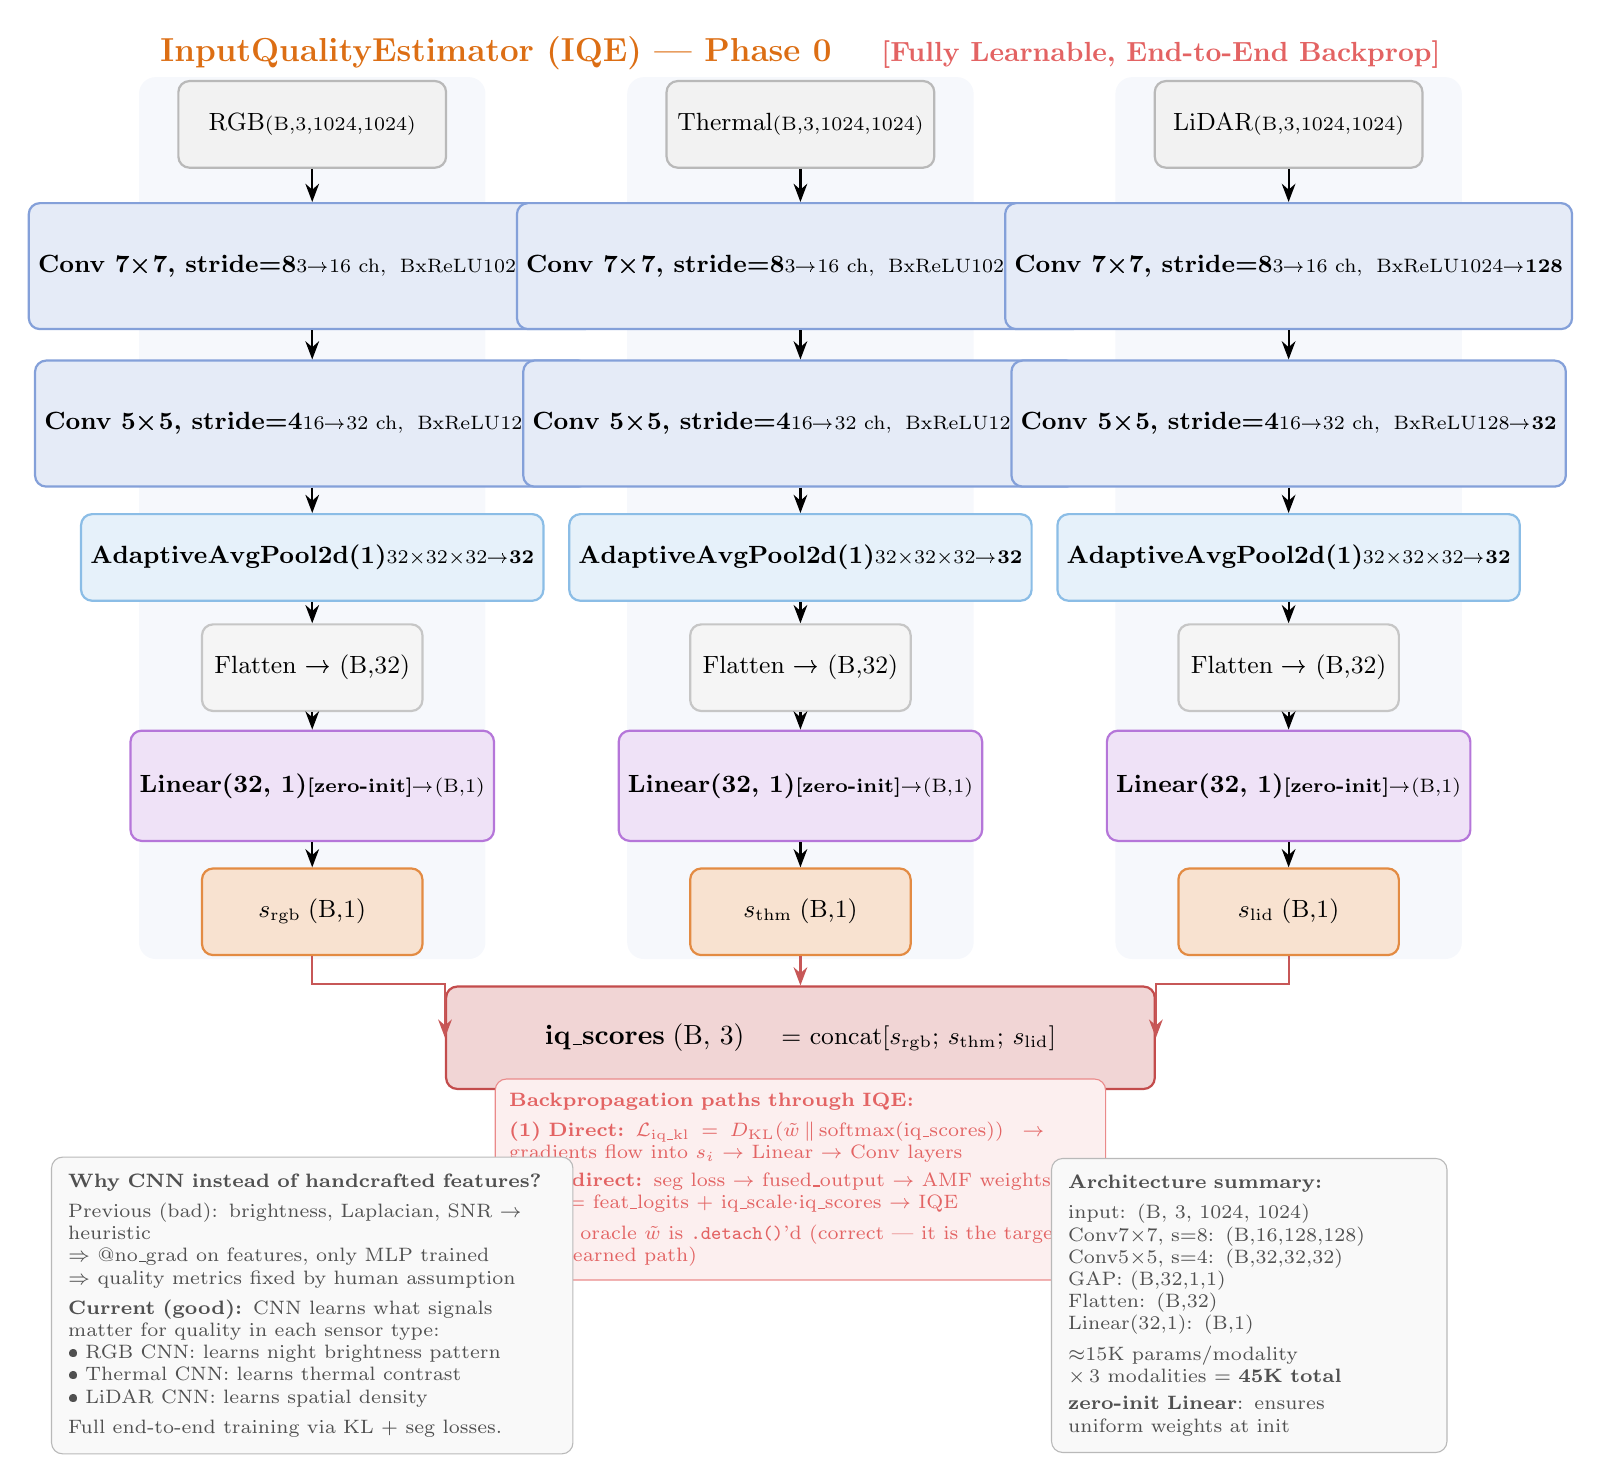
\begin{tikzpicture}

%% ══════════════════════════════════════════
%%  Column centers x = 2.6,  8.8,  15.0
%%  Row tops (y) — same for all columns:
%%    y =  0.0   input header
%%    y = -1.6   Conv 7×7 s=8
%%    y = -3.2   Conv 5×5 s=4
%%    y = -4.8   GAP
%%    y = -6.2   Flatten
%%    y = -7.6   Linear(32,1)  [zero-init]
%%    y = -9.0   score output
%% ══════════════════════════════════════════

\node[font=\large\bfseries, text=cIQE] at (8.8, 0.9)
  {InputQualityEstimator (IQE) — Phase~0 \quad
   {\normalsize\color{cBP!80}[Fully Learnable, End-to-End Backprop]}};

%% ─── Column header (inputs) ───────────────────────────────────
\node[inp] (hR) at ( 2.6, 0.0) {RGB\\{\scriptsize(B,3,1024,1024)}};
\node[inp] (hT) at ( 8.8, 0.0) {Thermal\\{\scriptsize(B,3,1024,1024)}};
\node[inp] (hL) at (15.0, 0.0) {LiDAR\\{\scriptsize(B,3,1024,1024)}};

%% ─── Conv 7×7 stride=8 ────────────────────────────────────────
\node[convB, minimum height=16mm] (c1R) at ( 2.6,-1.8)
  {\textbf{Conv 7×7, stride=8}\\{\scriptsize 3→16 ch,\; BxReLU}\\{\scriptsize 1024→\textbf{128}}};
\node[convB, minimum height=16mm] (c1T) at ( 8.8,-1.8)
  {\textbf{Conv 7×7, stride=8}\\{\scriptsize 3→16 ch,\; BxReLU}\\{\scriptsize 1024→\textbf{128}}};
\node[convB, minimum height=16mm] (c1L) at (15.0,-1.8)
  {\textbf{Conv 7×7, stride=8}\\{\scriptsize 3→16 ch,\; BxReLU}\\{\scriptsize 1024→\textbf{128}}};

\draw[A] (hR)--(c1R);  \draw[A] (hT)--(c1T);  \draw[A] (hL)--(c1L);

%% ─── Conv 5×5 stride=4 ────────────────────────────────────────
\node[convB, minimum height=16mm] (c2R) at ( 2.6,-3.8)
  {\textbf{Conv 5×5, stride=4}\\{\scriptsize 16→32 ch,\; BxReLU}\\{\scriptsize 128→\textbf{32}}};
\node[convB, minimum height=16mm] (c2T) at ( 8.8,-3.8)
  {\textbf{Conv 5×5, stride=4}\\{\scriptsize 16→32 ch,\; BxReLU}\\{\scriptsize 128→\textbf{32}}};
\node[convB, minimum height=16mm] (c2L) at (15.0,-3.8)
  {\textbf{Conv 5×5, stride=4}\\{\scriptsize 16→32 ch,\; BxReLU}\\{\scriptsize 128→\textbf{32}}};

\draw[A] (c1R)--(c2R);  \draw[A] (c1T)--(c2T);  \draw[A] (c1L)--(c2L);

%% ─── GAP ──────────────────────────────────────────────────────
\node[poolB] (gpR) at ( 2.6,-5.5)
  {\textbf{AdaptiveAvgPool2d(1)}\\{\scriptsize 32$\times$32$\times$32→\textbf{32}}};
\node[poolB] (gpT) at ( 8.8,-5.5)
  {\textbf{AdaptiveAvgPool2d(1)}\\{\scriptsize 32$\times$32$\times$32→\textbf{32}}};
\node[poolB] (gpL) at (15.0,-5.5)
  {\textbf{AdaptiveAvgPool2d(1)}\\{\scriptsize 32$\times$32$\times$32→\textbf{32}}};

\draw[A] (c2R)--(gpR);  \draw[A] (c2T)--(gpT);  \draw[A] (c2L)--(gpL);

%% ─── Flatten ──────────────────────────────────────────────────
\node[BX, fill=gray!8, draw=gray!45, minimum width=28mm] (flR) at ( 2.6,-6.9)
  {Flatten → (B,32)};
\node[BX, fill=gray!8, draw=gray!45, minimum width=28mm] (flT) at ( 8.8,-6.9)
  {Flatten → (B,32)};
\node[BX, fill=gray!8, draw=gray!45, minimum width=28mm] (flL) at (15.0,-6.9)
  {Flatten → (B,32)};

\draw[A] (gpR)--(flR);  \draw[A] (gpT)--(flT);  \draw[A] (gpL)--(flL);

%% ─── Linear(32→1) [zero-init] ────────────────────────────────
\node[linB, minimum height=14mm] (lnR) at ( 2.6,-8.4)
  {\textbf{Linear(32, 1)}\\{\scriptsize \textbf{[zero-init]}}\\{\scriptsize→(B,1)}};
\node[linB, minimum height=14mm] (lnT) at ( 8.8,-8.4)
  {\textbf{Linear(32, 1)}\\{\scriptsize \textbf{[zero-init]}}\\{\scriptsize→(B,1)}};
\node[linB, minimum height=14mm] (lnL) at (15.0,-8.4)
  {\textbf{Linear(32, 1)}\\{\scriptsize \textbf{[zero-init]}}\\{\scriptsize→(B,1)}};

\draw[A] (flR)--(lnR);  \draw[A] (flT)--(lnT);  \draw[A] (flL)--(lnL);

%% ─── Quality score output ─────────────────────────────────────
\node[scoB] (sR) at ( 2.6,-10.0) {$s_\text{rgb}$\;(B,1)};
\node[scoB] (sT) at ( 8.8,-10.0) {$s_\text{thm}$\;(B,1)};
\node[scoB] (sL) at (15.0,-10.0) {$s_\text{lid}$\;(B,1)};

\draw[A] (lnR)--(sR);  \draw[A] (lnT)--(sT);  \draw[A] (lnL)--(sL);

%% ─── concat → iq_scores ───────────────────────────────────────
\node[outB] (IQ) at (8.8,-11.6)
  {\textbf{iq\_scores}\;(B, 3)
   \quad{\small $=$ concat$[s_\text{rgb};\,s_\text{thm};\,s_\text{lid}]$}};

\draw[A, cOut!80, thick]
  (sR.south) -- ++(0,-3.5mm) -| (IQ.west);
\draw[A, cOut!80, thick]
  (sT.south) -- (IQ.north);
\draw[A, cOut!80, thick]
  (sL.south) -- ++(0,-3.5mm) -| (IQ.east);

%% ─── Backprop annotation ──────────────────────────────────────
\node[bpB, text width=74mm] at (8.8,-13.4)
  {\textbf{Backpropagation paths through IQE:}\\[3pt]
   \textbf{(1) Direct:} $\mathcal{L}_\text{iq\_kl}
     = D_\text{KL}(\tilde{w}\,\|\,\text{softmax}(\text{iq\_scores}))$
   $\;\to\;$ gradients flow into $s_i$ $\to$ Linear $\to$ Conv layers\\[2pt]
   \textbf{(2) Indirect:} seg loss $\to$ fused\_output
   $\to$ AMF weights $\to$ logits $= $ feat\_logits $+$ iq\_scale$\cdot$iq\_scores
   $\to$ IQE\\[3pt]
   \textbf{Note:} oracle $\tilde{w}$ is \texttt{.detach()}'d (correct — it is the target, not a learned path)};

%% ─── Design principle note ────────────────────────────────────
\node[noteB, text width=62mm] at (2.6,-15.0)
  {\textbf{Why CNN instead of handcrafted features?}\\[3pt]
   Previous (bad): brightness, Laplacian, SNR $\to$ heuristic\\
   $\Rightarrow$ @no\_grad on features, only MLP trained\\
   $\Rightarrow$ quality metrics fixed by human assumption\\[3pt]
   \textbf{Current (good):} CNN learns what signals\\
   matter for quality in each sensor type:\\
   \textbullet\;RGB CNN: learns night brightness pattern\\
   \textbullet\;Thermal CNN: learns thermal contrast\\
   \textbullet\;LiDAR CNN: learns spatial density\\[3pt]
   Full end-to-end training via KL + seg losses.};

\node[noteB, text width=46mm] at (14.5,-15.0)
  {\textbf{Architecture summary:}\\[3pt]
   input: (B, 3, 1024, 1024)\\
   Conv7$\times$7, s=8: (B,16,128,128)\\
   Conv5$\times$5, s=4: (B,32,32,32)\\
   GAP: (B,32,1,1)\\
   Flatten: (B,32)\\
   Linear(32,1): (B,1)\\[3pt]
   $\approx$15K params/modality\\
   $\times\,3$ modalities = \textbf{45K total}\\[2pt]
   \textbf{zero-init Linear}: ensures\\
   uniform weights at init};

%% ─── Column backgrounds ───────────────────────────────────────
\begin{scope}[on background layer]
  \fill[cConv!5, rounded corners=6pt]
    (0.4,  0.6) rectangle (4.8,-10.6);
  \fill[cConv!5, rounded corners=6pt]
    (6.6,  0.6) rectangle (11.0,-10.6);
  \fill[cConv!5, rounded corners=6pt]
    (12.8, 0.6) rectangle (17.2,-10.6);
\end{scope}

\end{tikzpicture}
\end{document}
